%%%%%%%%%%%%%%%%%%%%%%%%%%%%%%%%%%%%%%%%%
% a0poster Portrait Poster 
% LaTeX Template
% with University Copenhagen logo
% Version 1.0 (22/06/13)
%
% Based on:
% The a0poster class was created by:
% Gerlinde Kettl and Matthias Weiser (tex@kettl.de)
% 
% This template has been downloaded from:
% http://www.LaTeXTemplates.com
%
%%%%%%%%%%%%%%%%%%%%%%%%%%%%%%%%%%%%%%%%%

%----------------------------------------------------------------------------------------
%	PACKAGES AND OTHER DOCUMENT CONFIGURATIONS
%----------------------------------------------------------------------------------------

\documentclass[a0,portrait]{a0poster}
\usepackage[utf8]{inputenc}

\usepackage{multicol} % This is so we can have multiple columns of text side-by-side
\columnsep=100pt % This is the amount of white space between the columns in the poster
\columnseprule=3pt % This is the thickness of the black line between the columns in the poster

\usepackage[svgnames]{xcolor} % Specify colors by their 'svgnames', for a full list of all colors available see here: http://www.latextemplates.com/svgnames-colors

\usepackage{times} % Use the times font
%\usepackage{palatino} % Uncomment to use the Palatino font
\usepackage{array}
\usepackage{graphicx} % Required for including images
\usepackage{subcaption} 
\graphicspath{{figures/}} % Location of the graphics files
\usepackage{booktabs} % Top and bottom rules for table
\usepackage[font=small,labelfont=bf]{caption} % Required for specifying captions to tables and figures
\usepackage{amsfonts, amsmath, amsthm, amssymb} % For math fonts, symbols and environments
\usepackage{wrapfig} % Allows wrapping text around tables and figures

\usepackage{hyperref}
\hypersetup{colorlinks=true,
	citecolor=black,
	linkcolor=black, % links to parts of the document (e.g. index) in black
	urlcolor=blue} % links to resources outside the document in blue

\definecolor{ku}{RGB}{144,26,30}
\definecolor{ku-yellow}{RGB}{255,249,25}

 \usepackage{eso-pic}
               \newcommand\BackgroundIm{
               \put(66,-71){
               \parbox[b][\paperheight]{\paperwidth}{%
               \vfill
               \centering
               \includegraphics[height=\paperheight,width=\paperwidth,
               keepaspectratio]{UWTSD-house.pdf}%
               \vfill
               }}}

\begin{document}
\AddToShipoutPicture*{\BackgroundIm}
%----------------------------------------------------------------------------------------
%	POSTER HEADER 
%----------------------------------------------------------------------------------------

% The header is divided into two boxes:
% The first is 75% wide and houses the title, subtitle, names, university/organization and contact information
% The second is 25% wide and houses a logo for your university/organization or a photo of you
% The widths of these boxes can be easily edited to accommodate your content as you see fit



\begin{minipage}[t]{0.60\linewidth}
	\vspace{9.5cm}
	\Huge \color{ku} \textbf{A Risky Coexistence: Examining the Challenges Faced by Autonomous Vehicles and Motorcycles} \color{Black}\\ % Title
	\huge\textit{Research of the Enhancing Self-Driving Car Performance: The
		Potential Dangers of Autonomous Vehicles and Motorcycles}\\[1cm] % Subtitle
	\Large \textbf{Edward S. R. Patch (1801492)}\\[0.5cm] % Author(s)
	\Large Software Engineering and Artificial Intelligence\\[0.4cm] % University/organization

\end{minipage}
%
\begin{minipage}[t]{0.40\linewidth}
	\vspace{9.5cm}
	\flushright
	\color{DarkSlateGray}
	\Large \textbf{Contact Information:}\\
	Waterfront IQ Campus\\
	University of Wales Trinity,\\
	Swansea, SA1 8EW.\\[1cm]
	Email: \texttt{1801492@student.uwtsd.ac.uk} % Email address
\end{minipage}

\vspace{1cm} % A bit of extra whitespace between the header and poster content

%----------------------------------------------------------------------------------------

\begin{multicols}{2} % This is how many columns your poster will be broken into, a portrait poster is generally split into 2 columns

	%----------------------------------------------------------------------------------------
	%	ABSTRACT
	%----------------------------------------------------------------------------------------

	\color{ku} % Navy color for the abstract

	\begin{abstract}

	\end{abstract}

	%----------------------------------------------------------------------------------------
	%	INTRODUCTION
	%----------------------------------------------------------------------------------------

	\color{DarkRed} % SaddleBrown color for the introduction

    \section*{Introduction}
        Autonomous Vehicles (AVs) are scheduled to roll out to the United Kingdom roads by 2025.~\cite{govuk_self-driving_2022} With the rise of automated vehicles, a safety concern arises, which affects the development of AVs, including government bodies and manufacturers, public safety and the National Health Service (NHS), when it comes to motorcycles and AVs. The research focuses on issues that may have been overlooked already with motorcycles, with new scenarios introduced in many US states, like road widths, filtering and poor weather conditions with British vehicles. 

        Addressing these issues could be problematic; however, with Object Classification, which is not entirely accurate compared to AV standard, the research could push more extensive research in this area. The study's objectives are to understand the existing dangers with AVs and motorcycles, establish appropriate datasets to train and test the selected models, remove any vehicles that are not necessary for the study, and evaluate the test results of the study.
        
        A few study results are showcased to illustrate the current issues that may arise, describing the reasoning the model may have not detected. These results will be cross-referenced to research that did similar tests to support the argument to drive the safety issues that may still exist with AV manufacturers or newly established UK AV manufacturers.
	
	%----------------------------------------------------------------------------------------
	%	OBJECTIVES
	%----------------------------------------------------------------------------------------

	\color{DarkSlateGray} % DarkSlateGray color for the rest of the content

	\section*{Main Objectives}
		\begin{enumerate}
			\item Understanding of what dangers exist with AVs and motorcycles.
			\item Establishing the appropriate datasets to train and test the models.
			\item Pre-processing any datasets to improve the training progress.
			\item Evaluation of the test results to see specific information about where AVs may fail.
		\end{enumerate}

	%----------------------------------------------------------------------------------------
	%	MATERIALS AND METHODS
	%----------------------------------------------------------------------------------------

	\section*{Materials and Methods}
		\subsection*{Materials and Methods | Training}
			With the challenge of setting up a high-end model equivalent to a leading AV manufacturer like Tesla, it is essential to use detailed Object Classification training material. Using the Qualitative Research method with video frames and labels to classify the different objects in the video is required. Roboflow and other materials are outsourced and looked into using different sources found in various research journals.

			Using Python scripts, the selected training material is taken and processed together, allowing the model to see different motorcycles in different scenarios. A US and Indian dataset was used to get different road conditions and different types of motorcycles. Using the two datasets helped increase the accuracy during the validation process.

			Training of two datasets, dataset A with the filter of `bus', `car', `minivan', `motorcycle', `pickup', `scooter', `trike', `truck', `van', `person', whereas dataset B involves; `motorcycle', `tricycle' and `person' filters. The `yolov5s.pts' and `yolov5l.pts' were used during testing, with better results on the `yolov5l.pts' by 25\% when identifying motorcycles. Both weights used a batch of thirty-two and ten epochs.

		\subsection*{Materials and Methods | Testing}
			Testing materials must include video content, split into multiple frames To test the trained YOLO model, with enough images to create a strong argument. Joining a motorcycle group and exploring various routes across the United Kingdom, including motorways, dual carriageways, A-roads, and backroads, with motorcycles overtaking, filtering, and navigating blindspots, can lead to unexplored scenarios and questions that may have been previously overlooked.
					
			A decided factor is to use a Drift Innovation Ghost XL motorcycle camera attached to a motorcycle that rides within the group, then swap the camera with another rider after some time. This way, combining the content helps identify how Object Classification copes with numerous blindspots and draws some questions to further the research concerning the current safety of AV vehicles. 
			
			One sports bike and two cruisers are selected for material to test how Object Classification models handle different motorcycle styles. Ideal footage would include Scramblers, Trikes and other similar vehicles to establish how Object Classification models work in an estimated manner. A perfect material would be that during the ride out, conducted on 18$^\text{th}$ July 2023, Tuesday, would capture these vehicles, which either pass by or join us in sections of the rides. The group is instructed to overtake and be undertaken by the camera vehicle to create plenty of footage to put the YOLO model to the test. However, it is worth noting that no rider is pressured into doing anything illegal or unsafe.
	%----------------------------------------------------------------------------------------
	%	RESULTS 
	%----------------------------------------------------------------------------------------

	\section*{Results}
		\subsection*{Training Results}
			The large proved to be time-consuming to train the model with the size of the dataset, however, the result of dataset A scored a 81\% fitness on the motorcycle classification, where dataset B gathered a 77\% on the motorcycle classification.

			Confusion Matrix of Dataset A and Dataset B:
			\begin{center}\vspace{1cm}
				\begin{minipage}{0.2\textwidth}
					\centering
					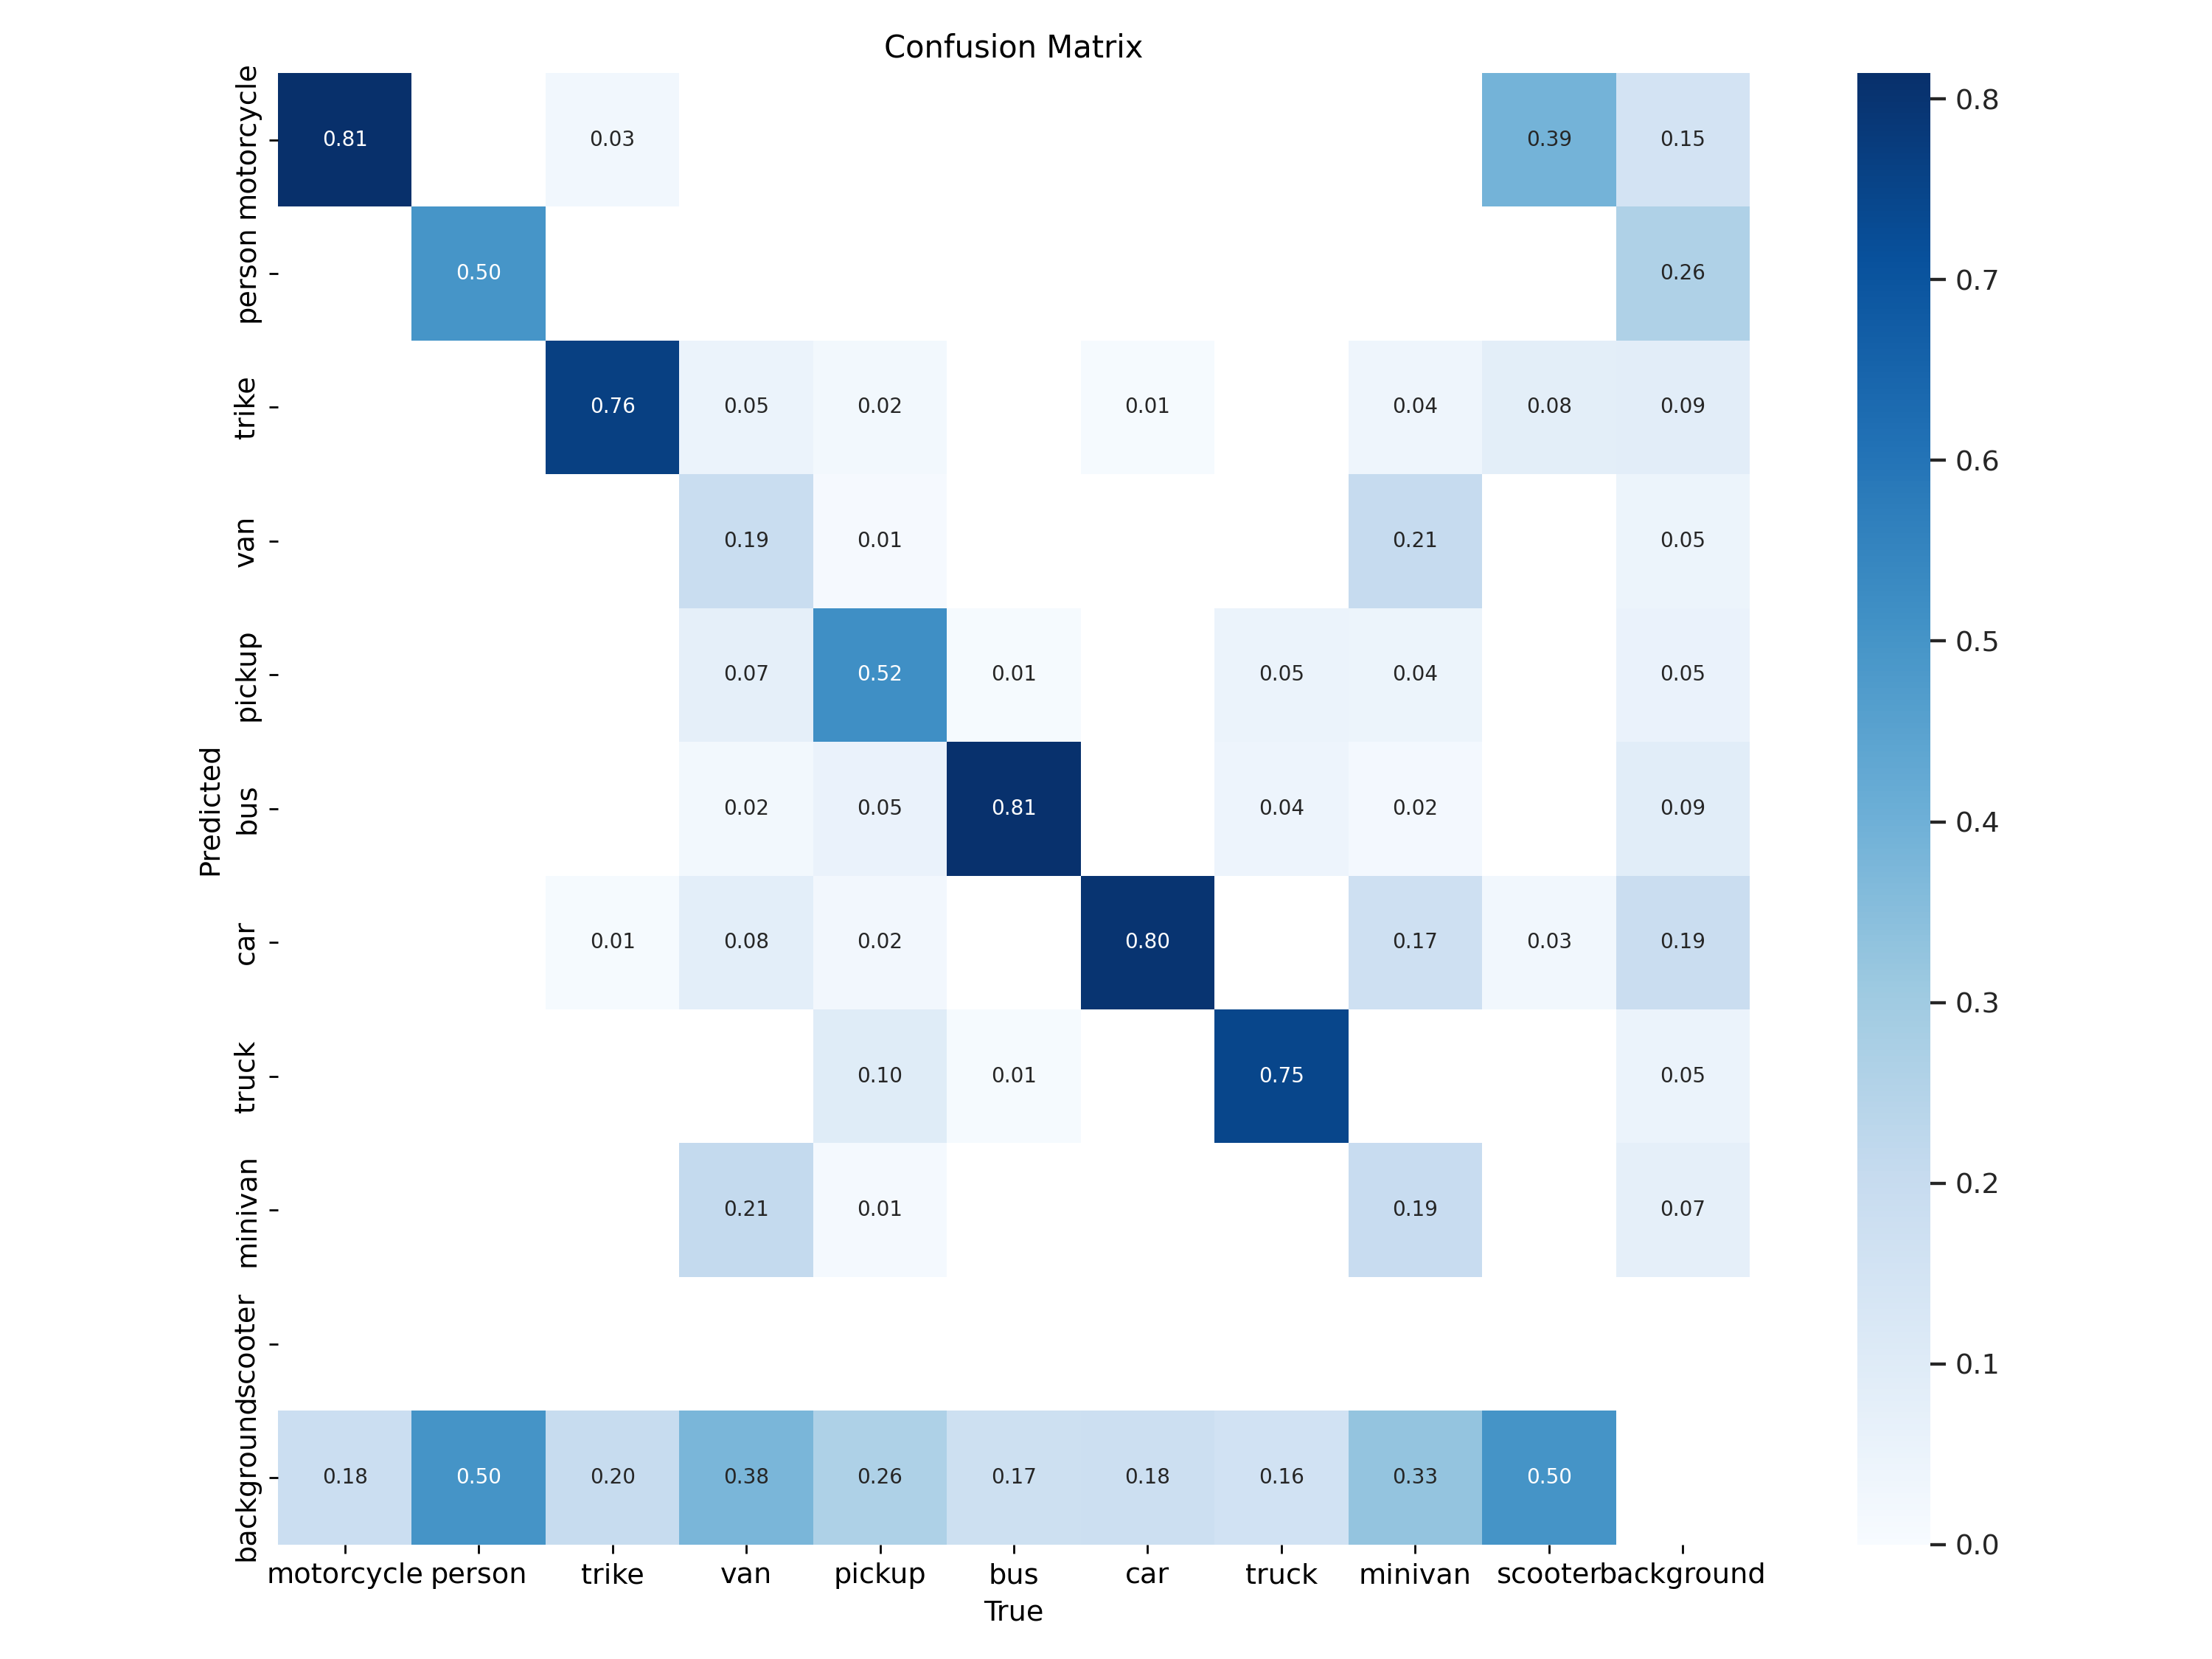
\includegraphics[width=\textwidth]{a_confusion_matrix.png}
					\captionof{figure}{\color{Green} Dataset A - Confusion Matrix}
					\label{fig:dAConfusionMatrix}
				\end{minipage}\hfill
				\begin{minipage}{0.2\textwidth}
					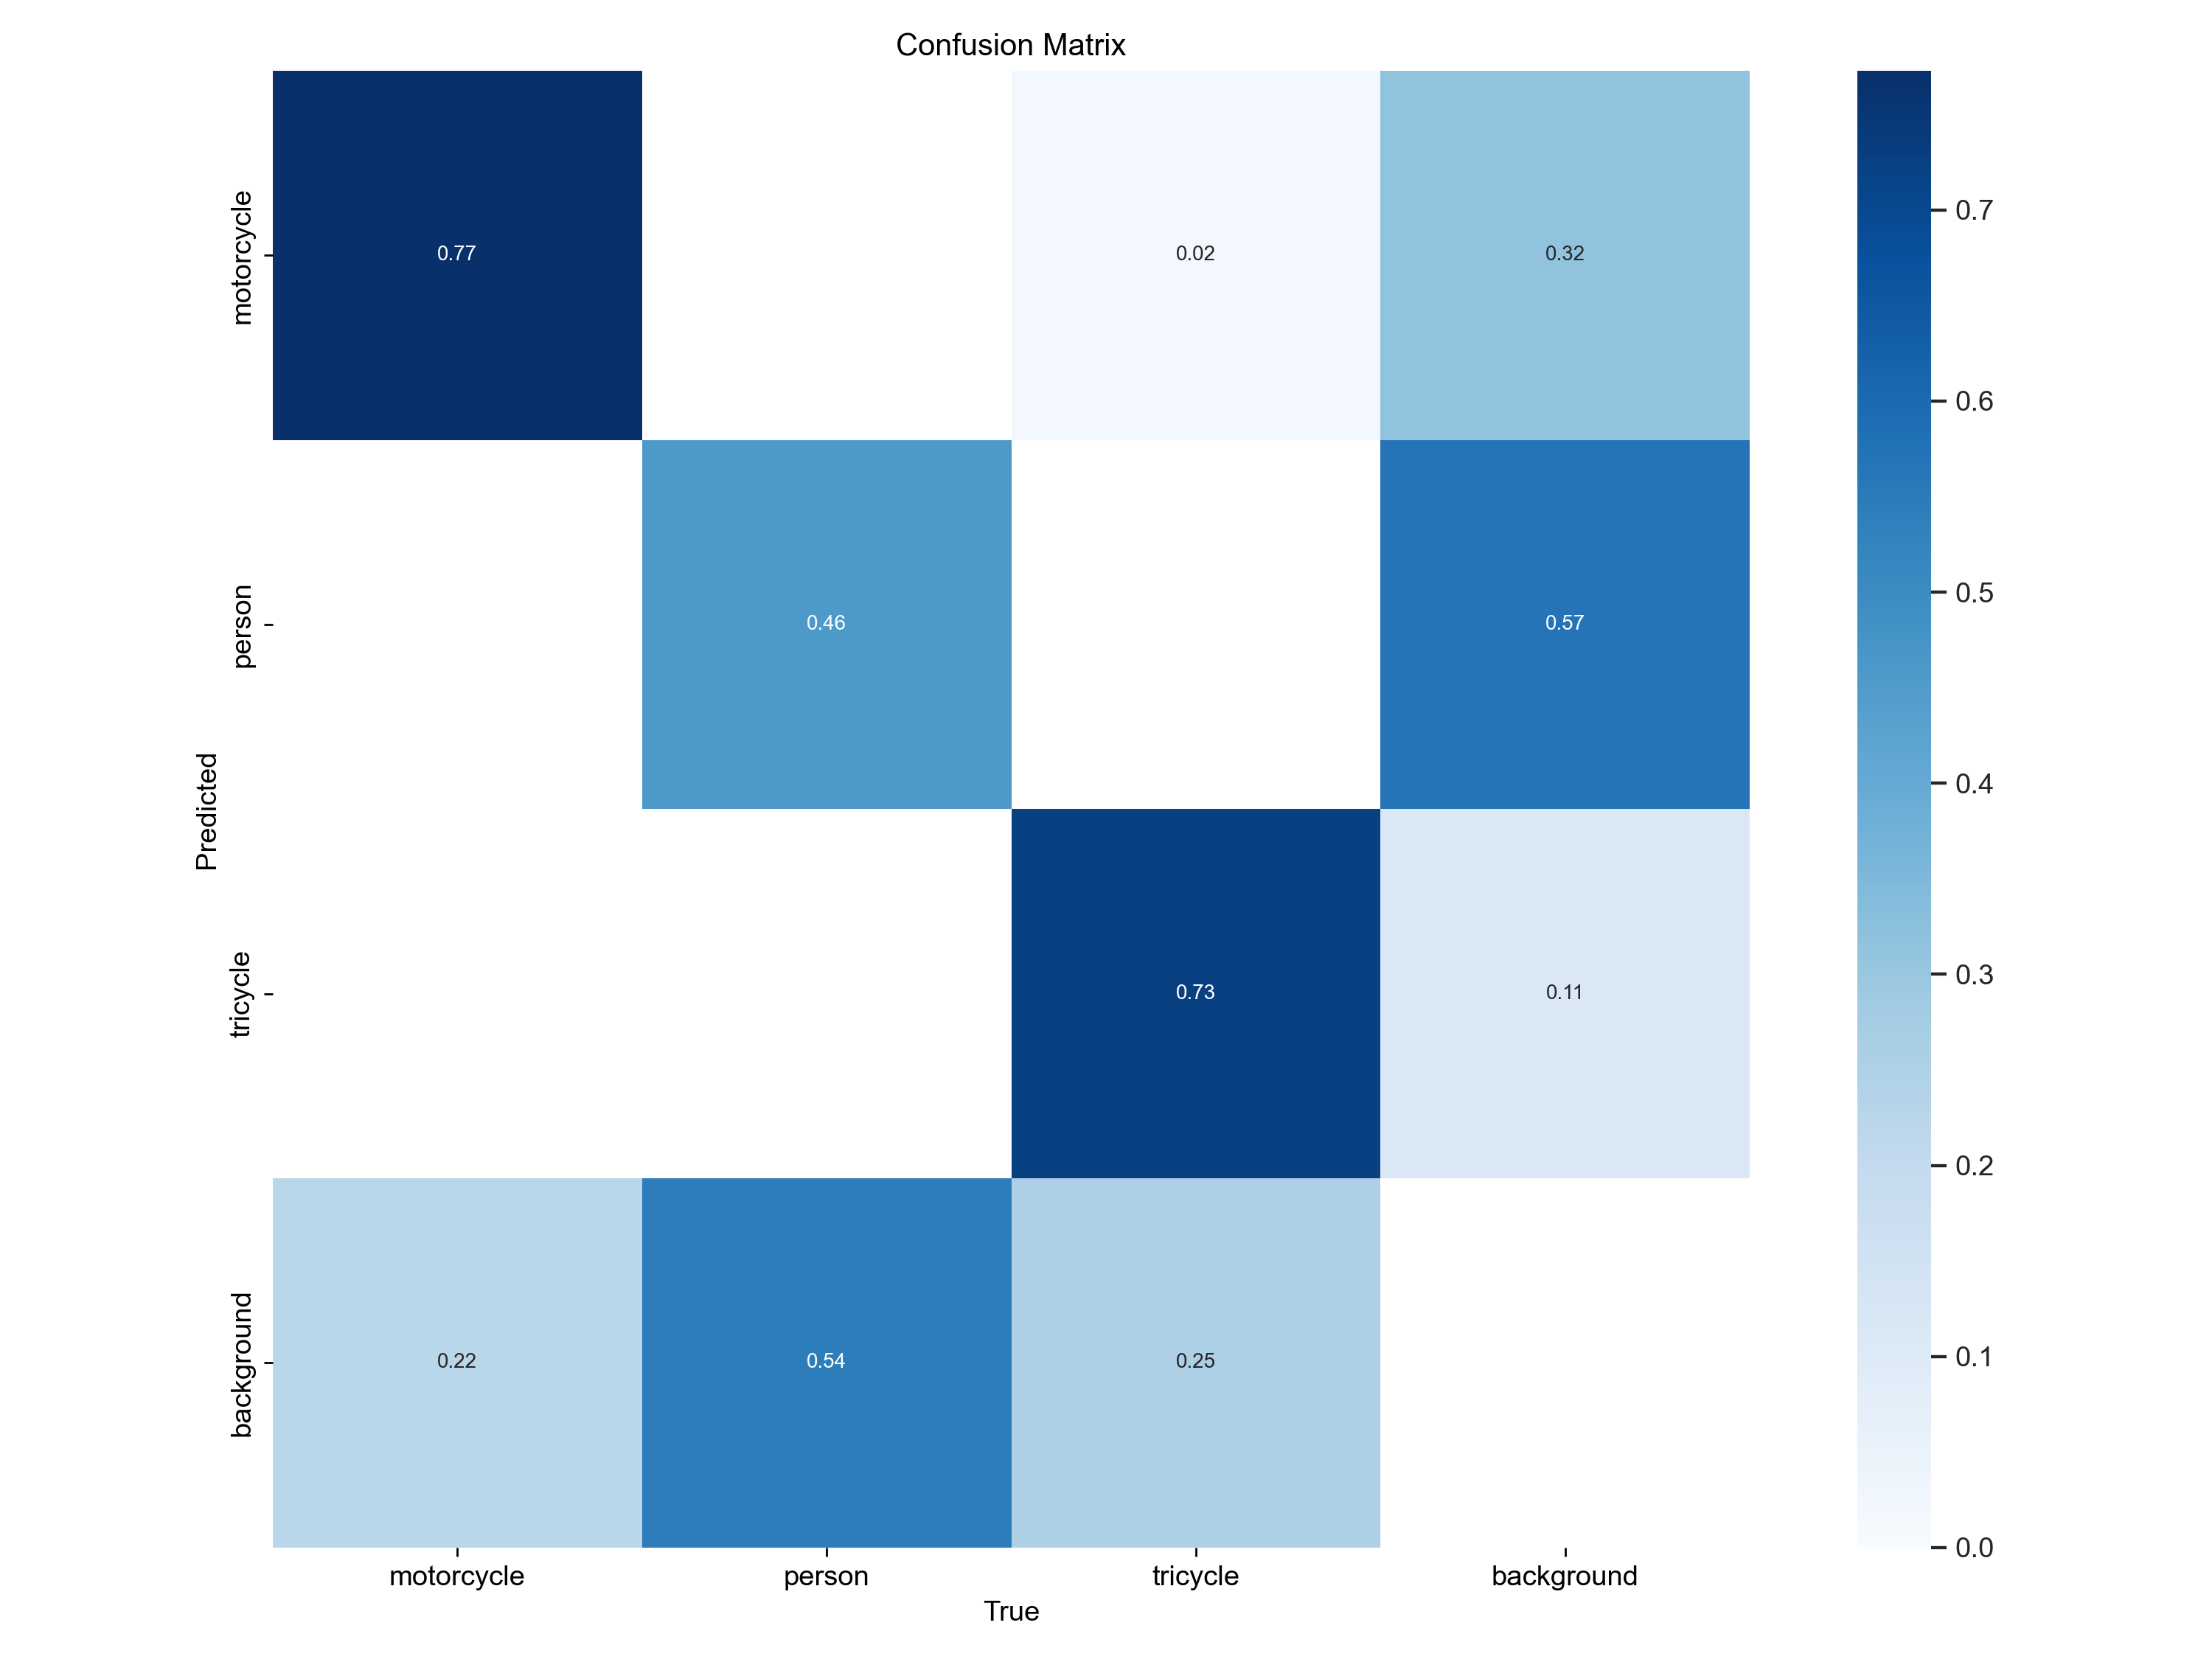
\includegraphics[width=\textwidth]{b_confusion_matrix.png}
					\captionof{figure}{\color{Green} Dataset B - Confusion Matrix}
					\label{fig:dBConfusionMatrix}
				\end{minipage}\vspace{1cm}
			\end{center}\vspace{1cm}

			

		\subsection*{Testing Results}
			The following images of~\ref{fig:detectionOfMotorcycleW1},~\ref{fig:detectionOfMotorcycleW2} and~\ref{fig:detectionOfMotorcycleW3} show different wet condition scenarios. Due to previous research conducted, according to Tesla, ``Tesla announces in 2021 that the company would remove a sensor called Ultrasonic Sensors, replacing the sensor with `Tesla Vision' by 2022''.~\cite{noauthor_tesla_nodate} This only means according to ``Self-Driving Cars and The Law: Putting autonomous vehicles on the road isn't just a matter of fine-tuning technology'' by Nathan A. Greenblatt, that AVs used `...thanks to lidar, radar, and ultrasonic sensors, they can see through fog and in the dark.', meaning that Tesla AVs for example, only use visual aid to see. However, this raises concerns about the reliability of Tesla's AVs that solely use visual input. For instance, in situations where the camera's view might be obscured by wet patches or heavy fog, a human driver could potentially outperform the technology.
			\begin{center}\vspace{1cm}
				\begin{minipage}{0.15\textwidth}
					\centering
					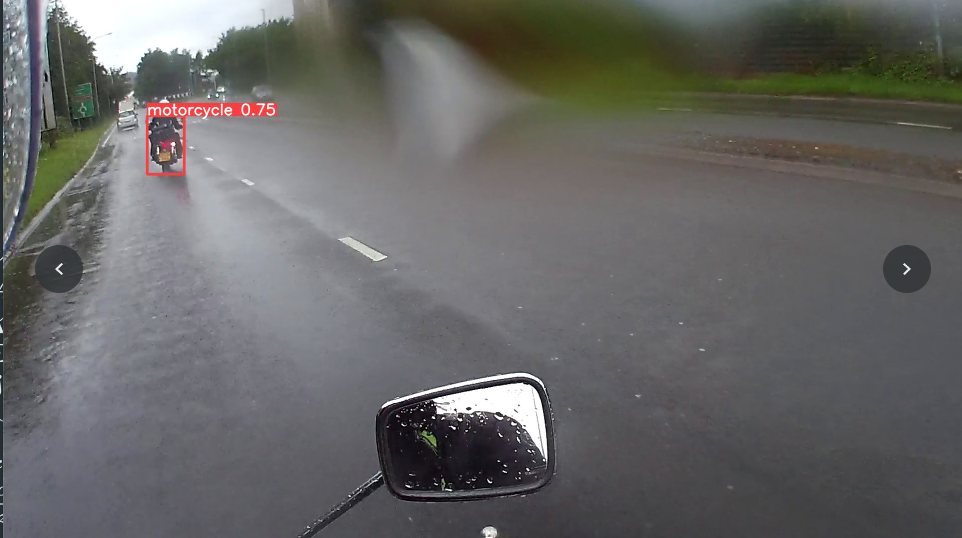
\includegraphics[width=\linewidth]{wet_correct.png}
					\captionof{figure}{\color{Green} Good Detection of Motorcycle - Wet and Multi Lane}
					\label{fig:detectionOfMotorcycleW1}
				\end{minipage}\hfill
				\begin{minipage}{0.15\textwidth}
					\centering
					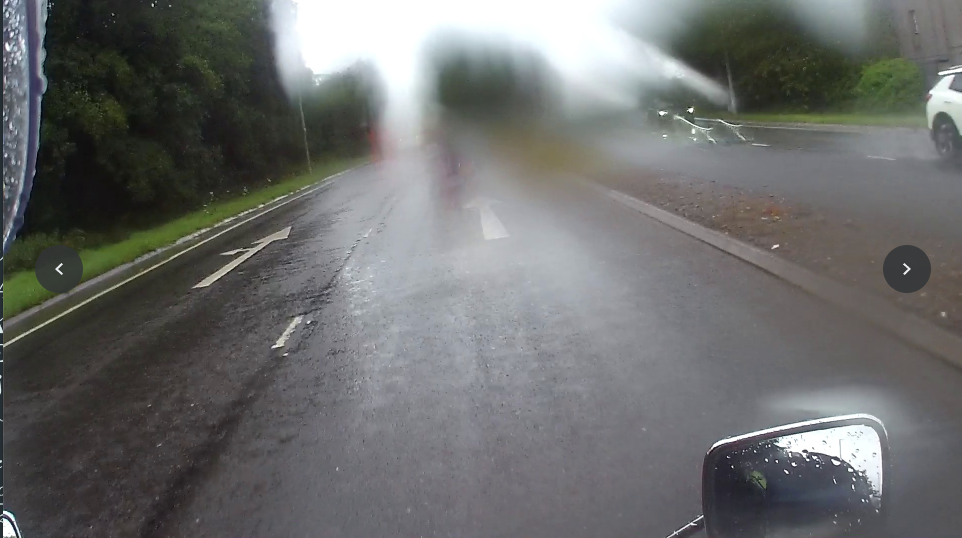
\includegraphics[width=\linewidth]{wet_incorrect.png}
					\captionof{figure}{\color{Green} Classification Error - Camera Blinded}
					\label{fig:detectionOfMotorcycleW2}
				\end{minipage}\hfill
				\begin{minipage}{0.15\textwidth}
					\centering
					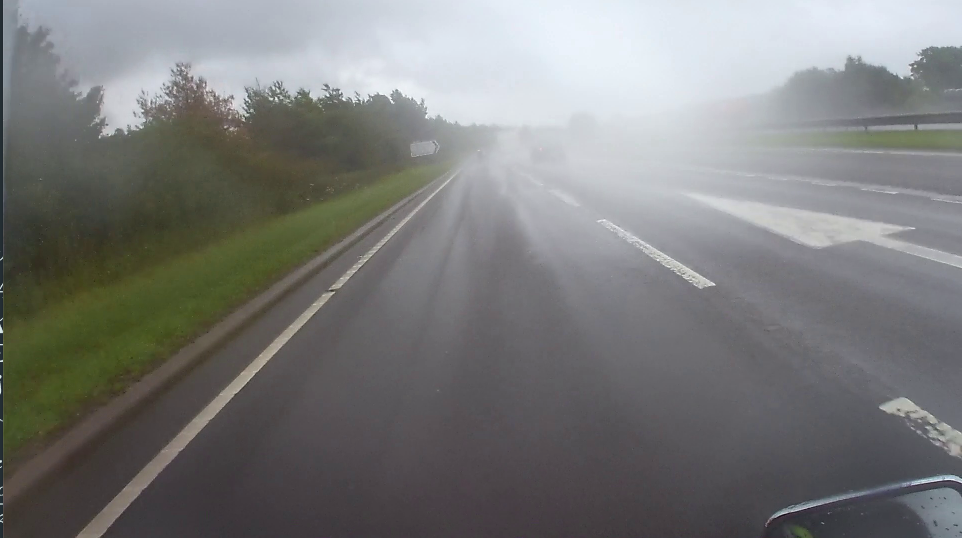
\includegraphics[width=\linewidth]{wet_danger.png}
					\captionof{figure}{\color{Green} Classification Error - Water Spray from Other Vehicles}
					\label{fig:detectionOfMotorcycleW3}
				\end{minipage}\vspace{1cm}
			\end{center}\vspace{1cm}
		
		A few examples of mis-classification errors; raises a serious question if a AV were to make a turn or a sudden movement, would this mean putting a motorcyclist in danger?
		\begin{center}\vspace{1cm}
			\begin{minipage}{0.15\textwidth}
				\centering
				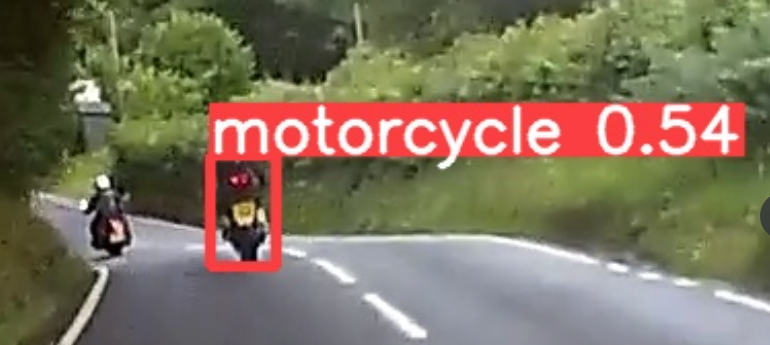
\includegraphics[width=\linewidth]{fail.png}
				\captionof{figure}{\color{Green} Detection of One Motorcycle}
				\label{fig:detectionOfOne}
			\end{minipage}\hfill
			\begin{minipage}{0.15\textwidth}
				\centering
				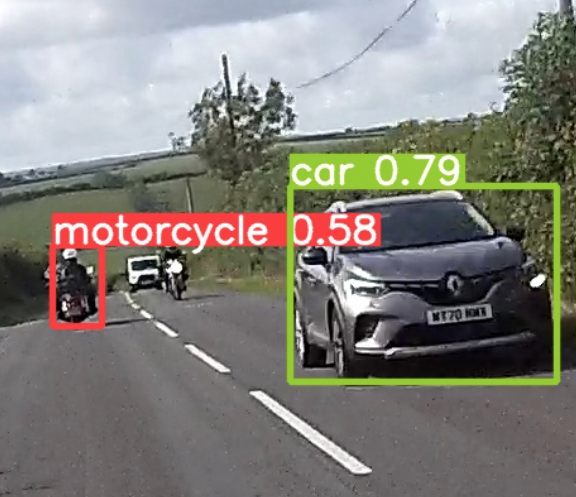
\includegraphics[width=\linewidth]{left_turn.png}
				\captionof{figure}{\color{Green} Late Classification - Part 1}
				\label{fig:lateClassificationP1}
			\end{minipage}\hfill
			\begin{minipage}{0.15\textwidth}
				\centering
				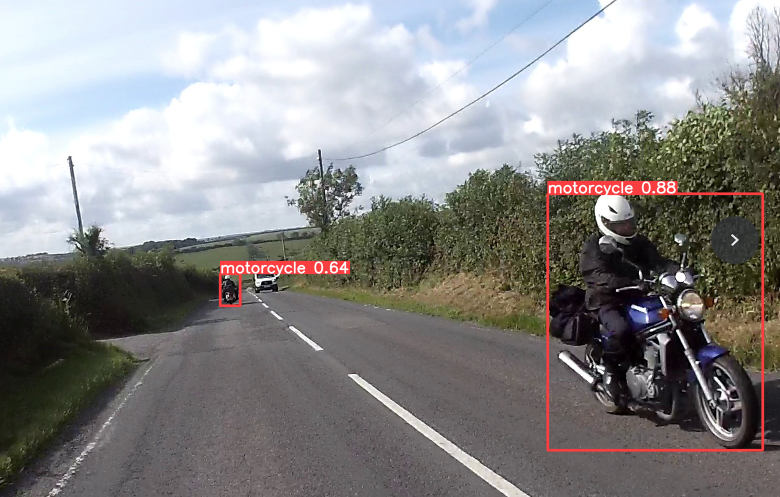
\includegraphics[width=\linewidth]{motorcycle.png}
				\captionof{figure}{\color{Green} Late Classification - Part 2}
				\label{fig:lateClassificationP2}
			\end{minipage}\vspace{1cm}
		\end{center}\vspace{1cm}

	%----------------------------------------------------------------------------------------
	%	CONCLUSIONS
	%----------------------------------------------------------------------------------------

	\color{DarkRed} % SaddleBrown color for the conclusions to make them stand out

	\section*{Conclusions}


	\color{DarkSlateGray} % Set the color back to DarkSlateGray for the rest of the content

	%----------------------------------------------------------------------------------------
	%	FORTHCOMING RESEARCH
	%----------------------------------------------------------------------------------------

	\section*{Forthcoming Research}

	%----------------------------------------------------------------------------------------
	%	REFERENCES
	%----------------------------------------------------------------------------------------

	\nocite{*} % Print all references regardless of whether they were cited in the poster or not
	\bibliographystyle{plain} % Plain referencing style
	\bibliography{ref} % Use the example bibliography file sample.bib

	%----------------------------------------------------------------------------------------
	%	ACKNOWLEDGEMENTS
	%----------------------------------------------------------------------------------------

	\section*{Acknowledgements}

	%----------------------------------------------------------------------------------------

\end{multicols}
\end{document}
